%%%%%%%%%%%%%%%%%%%%%%%%%%%%%%%%%%%%%%%%%%%%%%%%%%%%%%%%%%%%%%%%%%%%%%%%%%%%%%%%
\chapter{Разработка}
%%%%%%%%%%%%%%%%%%%%%%%%%%%%%%%%%%%%%%%%%%%%%%%%%%%%%%%%%%%%%%%%%%%%%%%%%%%%%%%%

Креатив.

%%%%%%%%%%%%%%%%%%%
\section{Подходы к проблеме}
%%%%%%%%%%%%%%%%%%%

***

%%%%%%%%%
\subsection{Нисходящий однопроходный метод}
%%%%%%%%%

Основная идея -- спуск по дереву разбора (CST) от корневого узла к листьям, собирая по пути следования информацию для определения контекста, в котором находятся обрабатываемые/инструментируемые узлы.
\nomenclature{CST}{Concrete Syntax Tree -- конкретное дерево разбора}

Обход "в глубину" (DFT).
\nomenclature{DFT}{Depth-First Traversal -- метод обхода графовой структуры, состоящий в том, чтобы идти ``вглубь'' графа, насколько это возможно}

***

Основная идея нисходящего подхода заключается в постепенном спуске по дереву разбора, которое генерирует внутри себя утилита TXL, от корневого узла к листьям, сохраняя по пути следования информацию для определения контекста, в котором находятся обрабатываемые узлы и выполняется инструментирование.

Ограничения:
\begin{itemize}
  \item Синтаксическое дерево исходного текста программы не содержит циклов по типам узлов -- при спуске от корня к листьям каждый тип узла встречается не более одного раза
\end{itemize}

%%%%%%%%%
\subsection{Нисходящий многопроходный метод}
%%%%%%%%%

***

%%%%%%%%%%%%%%%%%%%%%%%%%%%%%%%%%%%%%%%%%%%%%%%%%%%%%%%%%%%%%%%%%%%%%%%%%%%%%%%%
\section{Принцип работы системы инструментирования}
%%%%%%%%%%%%%%%%%%%%%%%%%%%%%%%%%%%%%%%%%%%%%%%%%%%%%%%%%%%%%%%%%%%%%%%%%%%%%%%%

***
Ключевыми идеями системы являются:
\begin{itemize}
  \item Оперирование контекстами инструментирования как некоторыми множествами.
  \item Использование одного прохода по дереву разбора для осуществления требуемых манипуляций (вставки фрагментов программного кода).
\end{itemize}

%%%%%%%%%%%%%%%%%%%
\subsection{Взаимодействие с окружением}
%%%%%%%%%%%%%%%%%%%

***

На рис.~\ref{fig:layout_artefacts} приведена обобщенная схема работы системы с позиции обрабатываемых и производимых артефактов, таких как файлы и аргументы командной строки (параметры запуска).

\begin{figure}[!h]
	\centering
	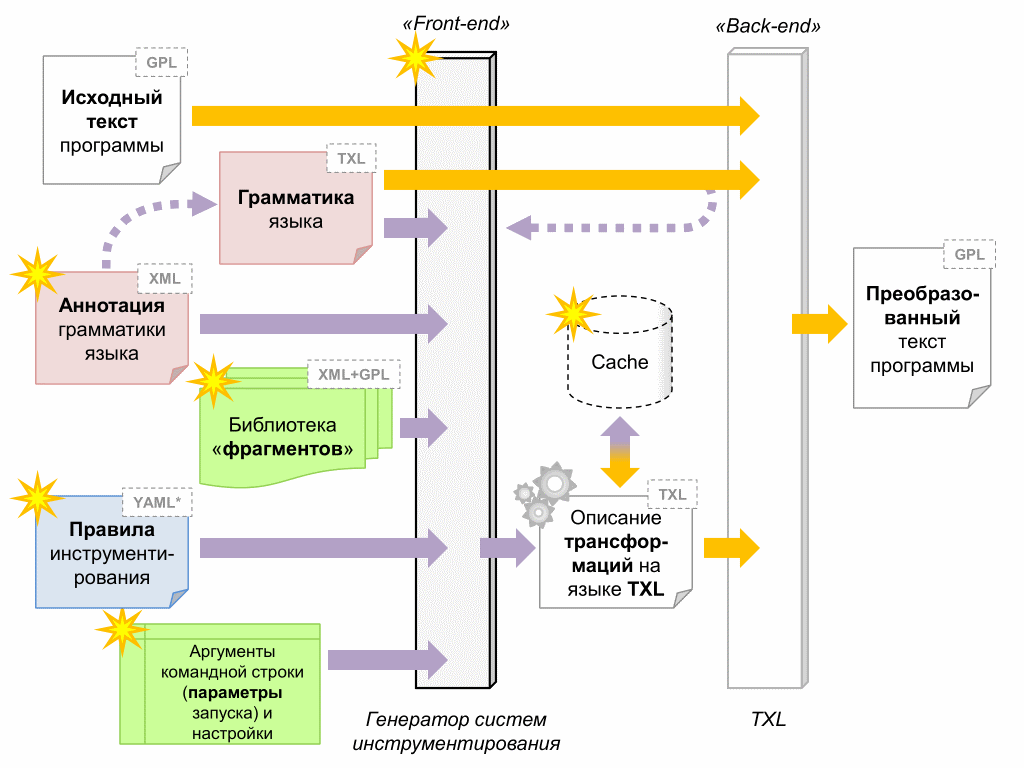
\includegraphics[width=4.2in]{layout_artefacts}
	\caption{Cхема работы системы. Артефакты.}
	\label{fig:layout_artefacts}
\end{figure}

для её работы необходимы:
\begin{itemize}
  \item Текст программы, инструментирование которой необходимо выполнить.
  \item Описание грамматики языка, на котором написан исходный текст этой программы.
  \item Аннотация грамматики языка.
  \item Пользовательские правила инструментирования.
  \item Фрагменты исходных текстов на выбранном языке программирования, вставку которых необбходимо выполнить.
  \item Дополнительные необязательные параметры запуска системы и переменные среды исполнения.
\end{itemize}

***

%%%%%%%%%%%%%%%%%%%
\subsection{Правила инструментирования}
%%%%%%%%%%%%%%%%%%%

***
про язык

Декларативный язык.

На рис.~\ref{fig:layout_ruleset} приведен пример описания правил инструментирования с точки зрения конечного пользователя системы.

\begin{figure}[!h]
	\centering
	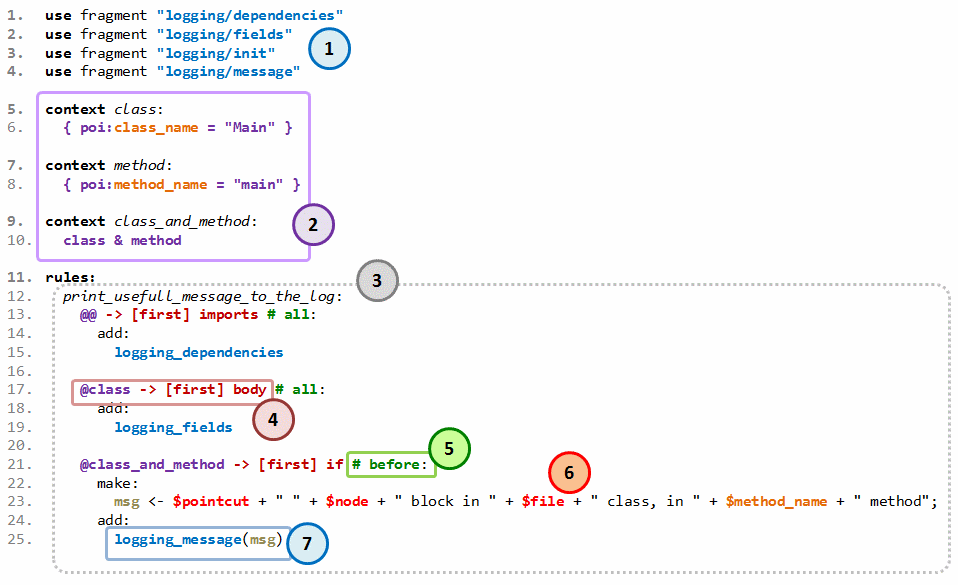
\includegraphics[width=4.2in]{layout_ruleset}
	\caption{Пример описания правил инструментирования}
	\label{fig:layout_ruleset}
\end{figure}

***

Основными частями пользовательского описания набора правил являются:
\begin{enumerate}
  \item перечисление используемых в данном наборе правил фрагментов исходных текстов и их относительное расположение в файловой системе;
  \item перечисление контекстов инструментирования;
  \item группировка этапов инструментирования в виде именованых правил;
  \item уточнение контекста инструментирования с применением ключевых слов языка программирования и текстовых шаблонов, если таковые требуются для целей уточнения контекста согласно решаемой пользователем задачи;
  \item указание одной конкретной точки инструментирования по ее идентификатору;
  \item создание пользовательских переменных из текстовых элементов и значений констант;
  \item список имен фрагментов, вставку которых необходимо выполнить одновременно в одном и том же месте, с указанием параметров, если таковые требуются согласно тексту используемого фрагмента.
\end{enumerate}

%%%%%%%%%%%%%%%%%%%
\subsection{Аннотация грамматики языка}
%%%%%%%%%%%%%%%%%%%

***
про XML

* Было бы удобно видеть в одном месте упрощенную схему иерархии типов узлов дерева разбора, в которой отображены только наиболее важные понятия языка программирования, для которого выполняется инструментирование, такие как \textit{класс}, \textit{метод}, \textit{оператор ветвления}, \textit{цикл со счетчиком} и др.

***

\begin{lstlisting}[frame=single, language=XML, label={annotation-dag-example}, caption={Пример}]
<!-- default pipeline: txl "%SRC%" "%TRANSFORM%" -o "%DST%" %PARAMS% -->
<annotation
  pipeline='txl "%SRC%" "%WORKDIR%\example\lang\python\pyindent.txl" | txl stdin "%TRANSFORM%" -o "%DST%" %PARAMS%'
  >
    <grammar
      language="python"
      src="lang\python\grammar.txl"
      >
        <keyword-DAG>
            <imports type="repeat statement_or_newline"/>
            <class type="classdef">
                <body type="statement_or_newline">
                    <method type="funcdef">
                        <if type="if_statement">
                            <elif type="elif_clause"/>
                            <else type="else_clause"/>
                        </if>
                        <for type="for_statement"/>
                        <while type="while_statement"/>
                        ...
                    </method>
                </body>
            </class>
        </keyword-DAG>
    </grammar>
...
\end{lstlisting}

***

\begin{lstlisting}[frame=single, language=XML, label={annotation-pois-example}, caption={Пример}]
<points-of-interest>
    <point
      id="class_name"
      keyword="class"
      value-of="classdef_head:id"
      />

    <point
      id="method_name"
      keyword="method"
      value-of="id"
      />

    <point
      id="if_condition"
      keyword="if"
      value-of="condition"
      />
...
\end{lstlisting}

***

\begin{lstlisting}[frame=single, language=XML, label={annotation-pointcuts-example}, caption={Пример}]
<pointcuts>
    <keyword
      name="method"
      search-type="funcdef"
      sequential="false"
      >
        <templates>
            <template kind="replace">
                'def <!--id--> <!--parameters--> ': 'INDENT <!--newline-->
                    <p name="before_body"/>
                    <!--repeat statement_or_newline-->
                    <p name="after_body"/>
                'DEDENT
            </template>

            <template kind="match">
                'def <!--id--> <!--parameters--> ': 'INDENT <!--newline-->
                    <!--repeat statement_or_newline-->
                'DEDENT
            </template>
        </templates>
        <pointcuts>
            <pointcut name="before_body" clone="if::before_body"/>

            <pointcut name="after_body">
                <paste-algorithm>
                    <fragment-to-variable
                      name="Additions"
                      type="repeat statement_or_newline"
                      each-line-postfix="Newline"
                      />
                    <insert-call
                      function="."
                      params="Additions"
                      />
                </paste-algorithm>
            </pointcut>
        </pointcuts>
    </keyword>
...
\end{lstlisting}

***

\begin{lstlisting}[frame=single, language=XML, label={annotation-template-example}, caption={Пример}]
<template kind="replace">
    'def <!--id--> <!--parameters--> ': 'INDENT <!--newline-->
        <p name="before_body"/>
        <!--repeat statement_or_newline-->
        <p name="after_body"/>
    'DEDENT
</template>
\end{lstlisting}

***

\begin{lstlisting}[frame=single, language=XML, label={annotation-algo-example}, caption={Пример}]
<pointcut name="before_body" clone="if::before_body"/>

<pointcut name="after_body">
    <paste-algorithm>
        <fragment-to-variable
          name="Additions"
          type="repeat statement_or_newline"
          each-line-postfix="Newline"
          />
        <insert-call
          function="."
          params="Additions"
          />
    </paste-algorithm>
</pointcut>
\end{lstlisting}

***

\begin{itemize}
  \item insert-text -- text
  \item insert-call -- function, params
  \item insert-fragment -- [each-line-prefix], [each-line-postfix]
  \item create-variable -- [name], type, value
  \item deconstruct-variable -- type, variant
  \item fragment-to-variable -- name, type, [each-line-prefix], [each-line-postfix]
\end{itemize}

***

\begin{lstlisting}[frame=single, language=XML, label={annotation-lib-example}, caption={Пример}]
<lib>
  <function
    name="addToImportsIfNotExists"
    apply="call"
    params="Addition:import_declaration"
    >
      <source>
        replace [repeat import_declaration]
          Imports [repeat import_declaration]

        deconstruct not * [import_declaration] Imports
          Addition

        by
          Imports [^ Addition]
      </source>
  </function>
...
\end{lstlisting}

***

%%%%%%%%%%%%%%%%%%%
\subsection{Фрагменты программного кода}
%%%%%%%%%%%%%%%%%%%

***
про XML

В листинге~\ref{fragment-example} приведен пример пользовательского параметризованного фрагмента программного кода на некотором целевом языке программирования (в данном случае -- Java).

\begin{lstlisting}[frame=single, language=XML, label={fragment-example}, caption={Пример пользовательского фрагмента}]
<fragment language="java" name="logging_message">
  <dependencies>
    <required name="logging_imports"/>
    <required name="logging_fields"/>
  </dependencies>

  <code black-list="imports" params="message">
    iLogger.log(Level.FINE, <p id="message"/>);
  </code>
</fragment>
\end{lstlisting}

***

%%%%%%%%%%%%%%%%%%%
\subsection{Пользователи системы}
%%%%%%%%%%%%%%%%%%%

На рис.~\ref{fig:layout_users} приведена схема работы системы инструментирования с позиции взаимодействия пользователей и системы как части производственного процесса (создания и отладки программного продукта).

\begin{figure}[h]
	\centering
	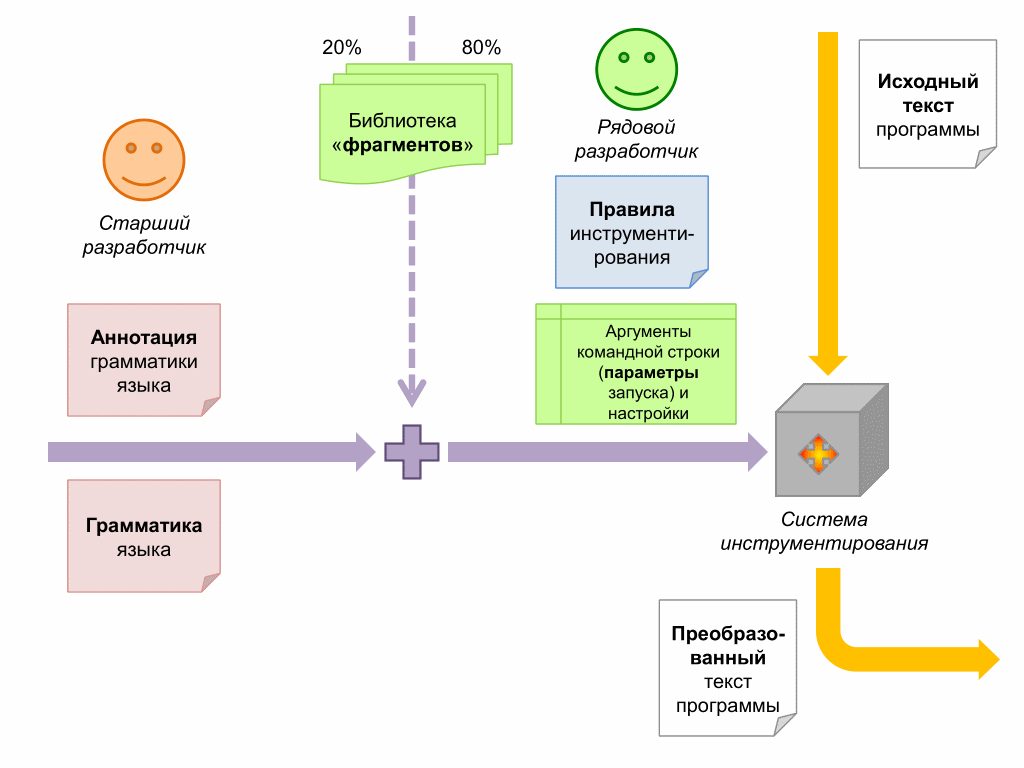
\includegraphics[width=4.2in]{layout_users}
	\caption{Cхема работы системы. Пользователи.}
	\label{fig:layout_users}
\end{figure}

***
с точки зрения пользователей есть два пользователя:

\begin{itemize}
  \item Разработчик грамматики -- более опытный пользователь, в лице старшего разработчика, в задачи которого входит:
    \begin{itemize}
      \item описание грамматики целевого языка программирования;
      \item составление аннотации к грамматике;
      \item отладка аннотации и грамматики;
      \item составление примеров фрагментов на целевом языке программирования.
    \end{itemize}

  \item Составитель правил инструментирования -- конечный пользователь, в лице рядового разработчика, в задачи которого входит:
    \begin{itemize}
      \item составление правил инструментирования;
      \item создание и пополнение библиотеки фрагментов исходных текстов на целевом языке;
      \item применение системы инструментирования к исходным текстам какой-либо программной системы.
    \end{itemize}
\end{itemize}

Исходя из задач, решаемых разными пользователями системы, можно выделить следующий минимальный набор компетенций для разных групп пользователей системы:
\begin{itemize}
  \item Разработчик грамматики:
    \begin{itemize}
      \item 1
    \end{itemize}

  \item Составитель правил инструментирования:
    \begin{itemize}
      \item 1
    \end{itemize}
\end{itemize}


%%%%%%%%%%%%%%%%%%%
\subsection{Выходные артефакты генератора}
%%%%%%%%%%%%%%%%%%%

***
про кэш и откат/копирование при ошибках

Исходя из предположения об использовании рассматриваемого генератора систем инструментирования как части процесса сборки некоторого промышленного программного обеспечения, которое имеет большой объем кодовой базы, можно сделать вывод о необходимости обеспечить разумный уровень сокращения повторяющихся ресурсо-затратных действий.

Наиболее ресурсо-затратными действиями при работе системы инструментирования будут следующие:
\begin{itemize}
  \item чтение каких-либо данных из файлового хранилища (жесткие диски, RAID-массивы жестких дисков);
  \item запись каких-либо данных в файловое хранилище;
  \item анализ и предобработка считанных данных;
  \item обработка и синтез выходных данных во временной памяти;
  \item запуск и ожидание других процессов операционной системы.
\end{itemize}
\nomenclature{RAID}{Redundant Array of Independent Disks -- технология виртуализации данных для объединения физических дисковых устройств}

С учетом относительного времени, которое необходимо для выполнения различных операций, приведенный список можно упорядочить следующим образом (меньше номер -- лучше):
\begin{enumerate}
  \item обработка и синтез выходных данных во временной памяти;
  \item анализ и предобработка считанных данных;
  \item чтение данных из файлового хранилища;
  \item запись данных в файловое хранилище;
  \item запуск и ожидание других процессов.
\end{enumerate}

Для простоты, примем время работы пунктов $1$ и $2$ одинаковым.

С учетом полученных результатов, рассмотрим более детально предполагаемый процесс инструментирования, изображенный на рисунке~\ref{fig:layout_artefacts}, уделяя внимание наиболее ресурсоемким выполняемым операциям.

Для генерации промежуточного описания трансформаций на языке TXL, генератору требуется выполнить \textbf{чтение} из файлового хранилища следующих артефактов:
\begin{itemize}
  \item грамматика целевого языка программирования;
  \item аннотация к грамматике;
  \item пользовательские правила инструментирования;
  \item несколько фрагментов из библиотеки фрагментов (зависимость от пользовательского описания, $N$).
\end{itemize}

Таким образом, генератор систем инструментирования должен выполнить $3 + N$ раздельных чтений из файлового хранилища, чтобы впоследствии выполнить \textbf{запись} в файловое хранилище промежуточного описания трансформаций и \textbf{запустить} утилиту TXL, которая в свою очередь выполнит несколько (минимум $3$, как видно на рис.~\ref{fig:layout_artefacts}) чтений и, как минимум, одну запись, в зависимости от сложности и структуры грамматики целевого языка программирования, для непосредственного инструментирования обрабатываемого исходного текста программы как часть завершающего этапа.

Исходя из специфики решаемой задачи, работы завершающего этапа необходимо выполнять для каждого файла исходного текста на целевом языке, содержащимся в кодовой базе инструментируемого ПО.
Таким образом, для оценки множества ресурсо-затратных действий, выполняемых системой инструментирования (генератор и утилита TXL), необходимо исключить из рассмотрения действия, выполняемые утилитой TXL, т.е. действия завершающего этапа инструментирования.

Помимо работы с файловым хранилищем, система инструментирования, в часности генератор, выполняет разбор и анализ загруженных данных, после чего обработку и синтез промежуточного описания правил трансформаций.
Перечисленные операции (разбор, анализ, обработка, синтез) производятся во временной памяти.

Следуя заключениям выше, составим общий объем работ, выполняемый

***

\nomenclature{SHA-1}{Secure Hash Algorithm 1 -- 160-битный алгоритм криптографического хэширования}
\nomenclature{MD5}{Message Digest 5 -- 128-битный алгоритм хэширования}

%%%%%%%%%%%%%%%%%%%%%%%%%%%%%%%%%%%%%%%%%%%%%%%%%%%%%%%%%%%%%%%%%%%%%%%%%%%%%%%%
\section{Выводы}
%%%%%%%%%%%%%%%%%%%%%%%%%%%%%%%%%%%%%%%%%%%%%%%%%%%%%%%%%%%%%%%%%%%%%%%%%%%%%%%%

Текст.
